\chapter{Introduction}
\epigraph{They're trying to understand what space is. That's tough for them.
They break distances down into concentrations of chemicals. For them, space is a
range of taste intensities.}{Greg Bear, Blood Music}
%
In order to meet the ever rising demand for computing speeds modern processor
architectures have become increasingly parallel and complex to circumvent
the inherent physical limitations of single core processors.
%
However, designing complex circuits is a difficult task, especially considering
the harsh demands on correctness, if even one in a billion instructions are
executed wrong the program will crash, or worse, give an incorrect result.
%
Nature on the other hand does not shy away from complexity, something the human
brain exemplifies:
%
Unlike the processor, it is not the result of some top down design
philosophy, yet through a process of self organization neurons are capable of
forming highly complex networks capable of solving complex tasks, with far
greater energy efficiency, robustness and parallellism than any designed
processor.
%
% Har dette nok med seksjonen over?
In order to investigate the processes that create the neural networks that makes
up the brain, a hybrid biological-digital robot has been created in a joint
multidisciplinary effort. 
%
Neurons are grown \emph{in vitro} on \emph{Micro Electrode Arrays}, shown in
figure \ref{neuroIntro} are interfaced with a digital computer throug lab
equipment (figure \ref{figEquipmentIntro}) which can perform highly accurate
voltage measurements forming a hybrid neuro-digital system. 
%
This system, known as a \emph{Cyborg}\footnote{A portmanteau word stemming from
  cybernetic organism} is used to control a small robot, allowing it to sense
and maneuver a simple maze.
%
The ultimate goal of the cyborg is to further our understanding of the
underlying principles that governing how nature computes.
%
\begin{figure}[h!]
  \centering
  \subfloat[an MEA]{{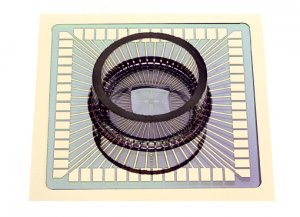
\includegraphics[width=5cm]{fig/MEA_front.jpg}}}%
  \qquad
  \subfloat[neural tissue on an MEA seen through a microscope]{{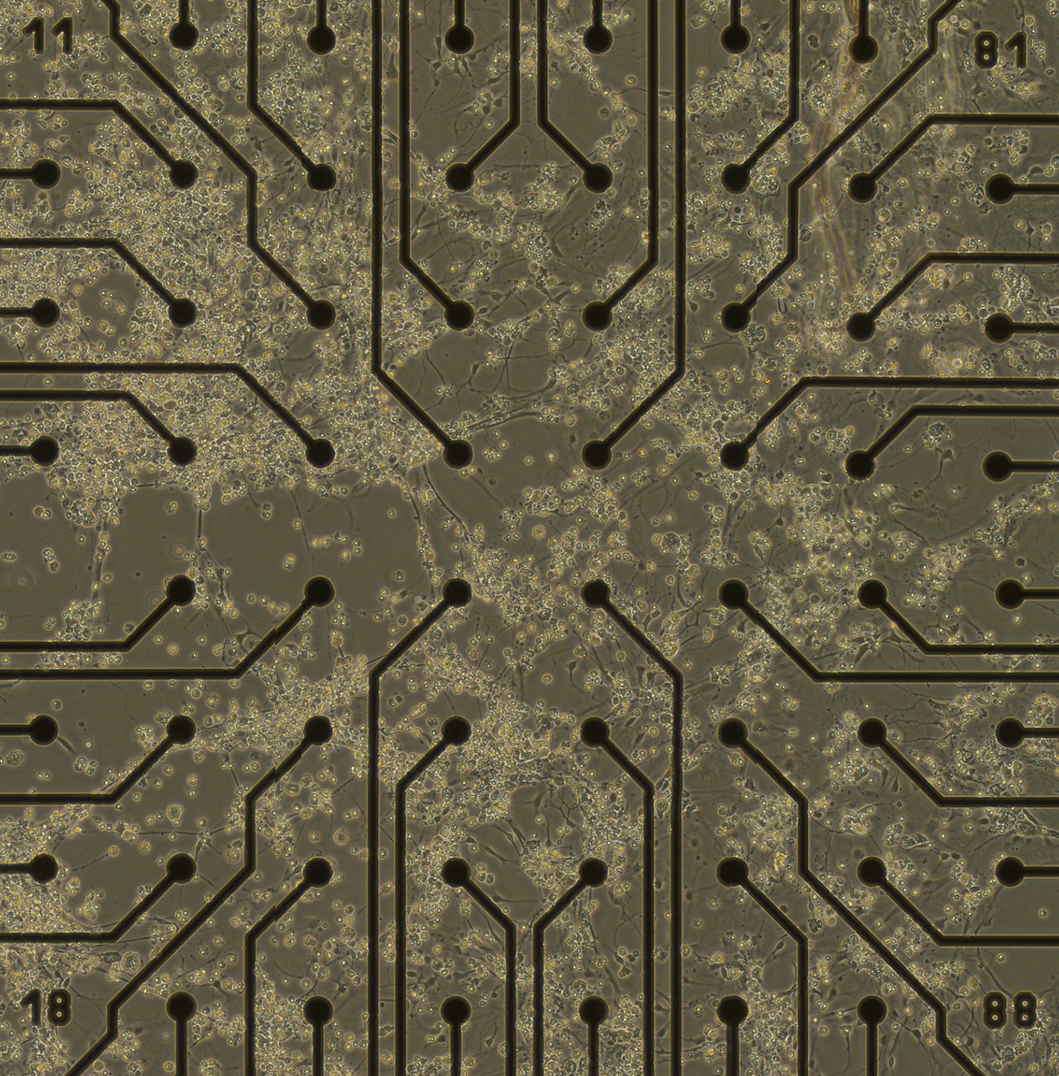
\includegraphics[width=5cm]{fig/frank.png}}}%
  \caption{
    A micro electrode array (MEA), lined with electrodes that extend to the
    middle chamber where neural tissue can be grown.
  }
  \label{neuroIntro}%
\end{figure}
%
%
\begin{figure}[h!]
  \centering
  \subfloat[An MEA2100 headstage]{{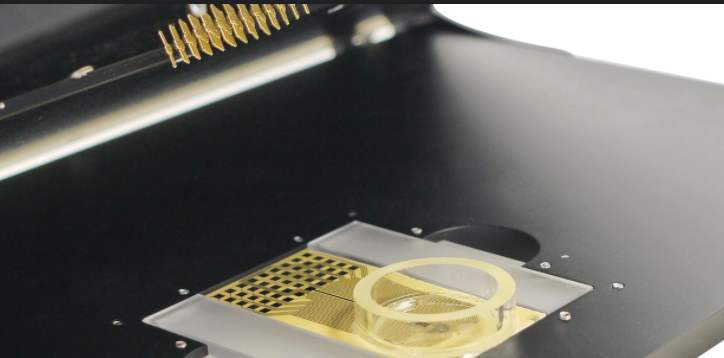
\includegraphics[width=5cm]{fig/hs_placeholder.png}}}%
  \qquad
  \subfloat[Electrical activity measured by a single electrode]{{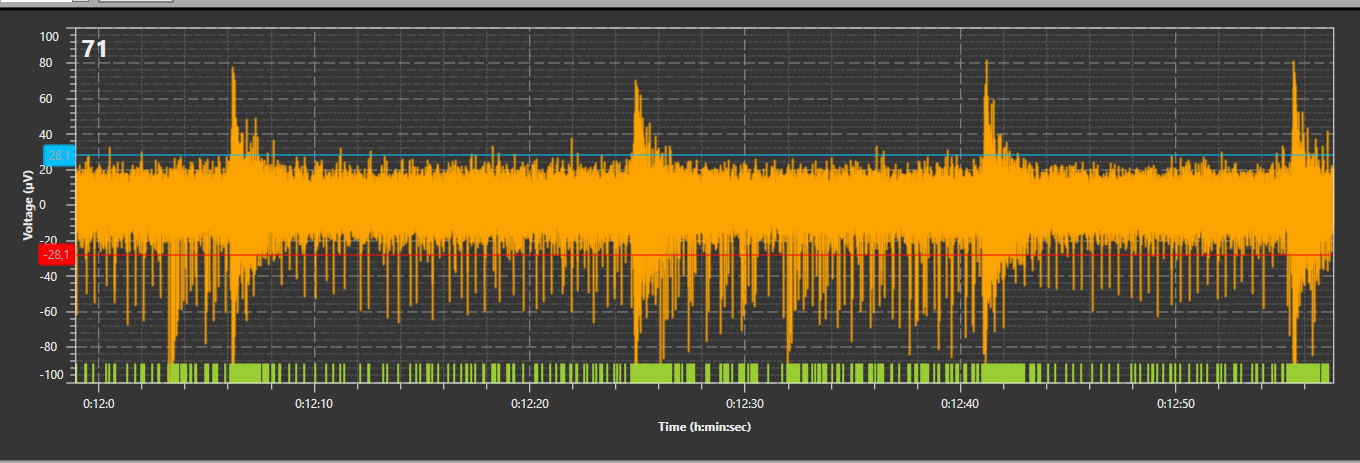
\includegraphics[width=5cm]{fig/PacemakerBurst.png}}}%
  \caption{
    MEAs containing neurons are inserted into equipment capable of measuring and
    inducing electrical activity at high precision.
  }
  \label{figEquipmentIntro}%
\end{figure}
\subsubsection{Complexity}
In the 50's and 60's there was much optimism in the burgeoning field of
artificial intelligence. In 1965 H. A. Simon claimed ``machines will be capable,
within twenty years, of doing any work a man can
do.''\cite{DREYFUS92} , while Marvin Minsky boldly claimed in 1967
that ``Within a generation [...] the problem of creating 'artificial intelligence'
will substantially be solved.'' \cite{DREYFUS92}.
Had they chosen to predict any other field, such as logistics, information
sharing or communications their statements would have been prophetic and
visionary, yet even today \emph{general artificial intelligence} seems no closer
to our grasp than it did 50 years ago, so why did artificial intelligence turn
out so differently? 
%
In their quest to make machines that could truly \emph{think}, being capable of
learning and reasoning about the world and solve problems they had never seen
before, the researchers sought to make machines that could apply logic similar
to that of high level human thinking.
%
It followed that the machine had to be programmed with rules governing logic in
order to reach sound conclusions, allowing it to store and manipulate its
knowledge of the world.
%
To represent the prior and deduced knowledge, the researchers designed
programming languages such as lisp\cite{LISP_WEENIE} that could accurately
describe these operations.
%
In order to actually execute these lisp programs, underlying hardware had to be
created, supporting the primitive operations such as addition, subtraction, and
loading from memory.
%
Regardless of the underlying platform, a lisp program did not change meaning,
separating execution and intent in an elegant manner allowing the programmer to
ignore implementation details.
%
In short, each piece of the puzzle was self contained, allowing the researchers 
to build large systems where each ``layer'' interacted in a manner that could be
reasoned about independendently, keeping the \emph{complexity} of the system in
check.
%
Nature, on the other hand, applies a completely different method.
Complex structures appear with no blueprint, arising from a process of
\emph{self-organization} driven by a set of growth rules.
%
This self-organizing process is capable of producing incredibly complex, robust
and diverse structures whose functionality arises not from specialized
components working in isolation, but from the interaction of many components.
%
The early AI researchers believed that to create an intelligent system it was
sufficient to provide a platform that could reason logically, but as history
shows this did not work out.
%
The human brain, however, is not hiding some underlying logic beneath incidental
complexity, instead it seems, the complexity itself might be the fundamental
driving force behind intelligence.
%
In short, intelligence does not arise from logic, instead our ability to reason
logically arises from intelligence, and focusing on the complex interaction of
neurons from which intelligence emerges could yield greater understanding of
just what intelligence actually is.
\subsubsection{Computation}
The invention of the digital computer will be remembered as one of, if not the
most significant technological advances of mankind.
%
With this neatly designed clockwork machine the concept of computation seemed
rather straight forward, where each executed machine instruction corresponded to
some unit of computation.
%
This idea of computation is very convenient, and it fails utterly when
applied to biological systems.
In a recent example of this from 2005 is Ray Kurzweils book The singularity is
near \cite{KURZWEIL2005}.
Ray Kurzweil claimed that computers would be as powerful as a
mouse brain by 2020, a prospect that looks rather unlikely in 2018.
Other than in the head of computer scientists, neurons have no notion of
floating point operations or branching logic, and measuring the computational
capabilities of a brain in FLOPS (a measure of raw throughput for primitive math
operations like addition and subtractions per second) is grossly underestimating
what computing \emph{can} be.
%
In spite of the digital computers shortcoming compared to the human brain, the
conventional digital approach to computing has been hugely successful in solving
problems that humans are bad at, and is so ubiquitus that other approaches
have been dubbed \emph{Unconventional Computing}.
%
Unconvential computing, as implied by the name, comes in many forms such as
buckets of water \cite{FERNANDO2003}, or blobs of carbon nanotubes
\cite{LYKKEBOICES2014}
%
In these unconventional approaches it becomes harder and harder to pin down
exactly what computation is and what distinguishes it from any ordinary physical
process.
\subsubsection{Cyborg}
The main body of work done for this thesis is the design and development of a as
part of the NTNU cyborg project\cite{ntnu_cyborg}, which comprises
researchers from the department of neuroscience, nano science, computer science,
cybernetics and more.
The work in this thesis is a continuation of the work performed by the cyborg
project \cite{TMAC}, 


Both by necessity and choice, most biological details are left out, the focal
point of the thesis is the system in which neural tissue is a part, not the
neurons themselves.
Thus only details that are necessary for the computational model of neural
tissue will be considered, leaving the intricate complexities of neurons to the
neuroscientists, at least for the time being.
\cleardoublepage

%%% Local Variables:
%%% mode: latex
%%% TeX-master: "../main"
%%% End:
